\chapter{Results}\label{chapter:results}

To quantify the influence of each \gls{vdp} on the performance of a baseline combination for a particular PBS performance measure, the coefficient of variation (\gls{cv}) metric was used. The \gls{cv} facilitates the comparison of datasets where the units of measurement may differ \cite{Soong2004} and is a measure of the spread of data about its mean.

Each \gls{vdp} was systematically varied in isolation with 5 equally distributed data points ranging from the minimum to the maximum value as per the ranges developed in Section~\ref{chapter:parameter-range-selection}. For each \gls{vdp}, the \gls{cv} of each PBS performance measure was calculated as per Equation~\ref{equation:cv}.

%----------------------------------------------
%      EQUATION
%----------------------------------------------
\begin{equation}
    \label{equation:cv}
    CV = \frac{\sigma}{\mu} \times 100\%
\end{equation}
%----------------------------------------------
%      EQUATION
%----------------------------------------------

To compare the relative influence of each \gls{vdp} on each \gls{pbs} performance measure, the \gls{cv} for each \gls{pbs} performance measure was normalised with respect to the parameter with the highest \gls{cv} ($CV_{max}$). Thus the \gls{cv} matrix columns are normalised according to $CV_{max}$ for that column and the normalised values are denoted as $CV_n$ as per Equation \ref{equation:cv-norm}.

%----------------------------------------------
%      EQUATION
%----------------------------------------------
\begin{equation}
    \label{equation:cv-norm}
    CV_{n} = \frac{CV}{CV_{max}} \times 100\%
\end{equation}
%----------------------------------------------
%      EQUATION
%----------------------------------------------

%----------------------------------------------
%      EQUATION
Where:
\begin{itemize}[label={}]
\item $\sigma$ = standard deviation for a single performance measure evaluated for a single \gls{vdp}
\item $\mu$ = mean performance for a single performance measure evaluated for a single \gls{vdp}
\item $CV$ = coefficient of variation for a single performance measure evaluated for a single \gls{vdp}
\item $CV_n$ = normalised coefficient of variation for a single performance measure evaluated for a single \gls{vdp}
\item $CV_{max}$ = maximum coefficient of variation observed for a single performance measure (each column in the \gls{cv} matrix represents a single performance measure)
\end{itemize}
%      EQUATION
%----------------------------------------------

Any parameter that produced a $CV_n$ of less than 10\% (i.e. a \gls{cv} less than 10\% of the maximum coefficient of variation for the same performance measure) for a performance measure was regarded as having a negligible relative influence and was omitted from the overall \gls{cv} matrices in Section~\ref{sec:results-overall}. A set of complete \gls{cv} matrices containing all evaluated \glspl{vdp} are included in Sections~\ref{section:complete-cv-quad-semi}~to~\ref{section:complete-cv-rigid-drawbar}. Additional matrices comparing the relative influence of the inertial, geometrical, suspension and tyre \glspl{vdp} in isolation can be found in Appendices~\ref{section:cv-geometrical}~to~\ref{section:cv-tyre}.

\section{Interpretation of the CV Matrix}\label{section:interpretation-of-the-results-matrix}

The columns of the \gls{cv} matrices represent \gls{pbs} performance measures and the rows represent \glspl{vdp}. The numerical value in a cell represents the \gls{cvn} for the \gls{vdp} described in that row with respect to the \gls{pbs} performance described in that column.

In a single column, the influence of each \gls{vdp} on a \gls{pbs} performance measure is recorded relative to the \gls{vdp} that had the maximum influence on the \gls{pbs} performance measure according to Table~\ref{table:cv-matrix-conventions}. Each row indicates the relative influence of the described \gls{vdp} on each of the \gls{pbs} performance measures. An example of interpreting the \gls{cv} matrices is provided in Figure~\ref{figure:interpretation-of-cv-matrix}.

%----------------------------------------------
%      FIGURE
%----------------------------------------------
    \begin{figure}[H]
        \centering
        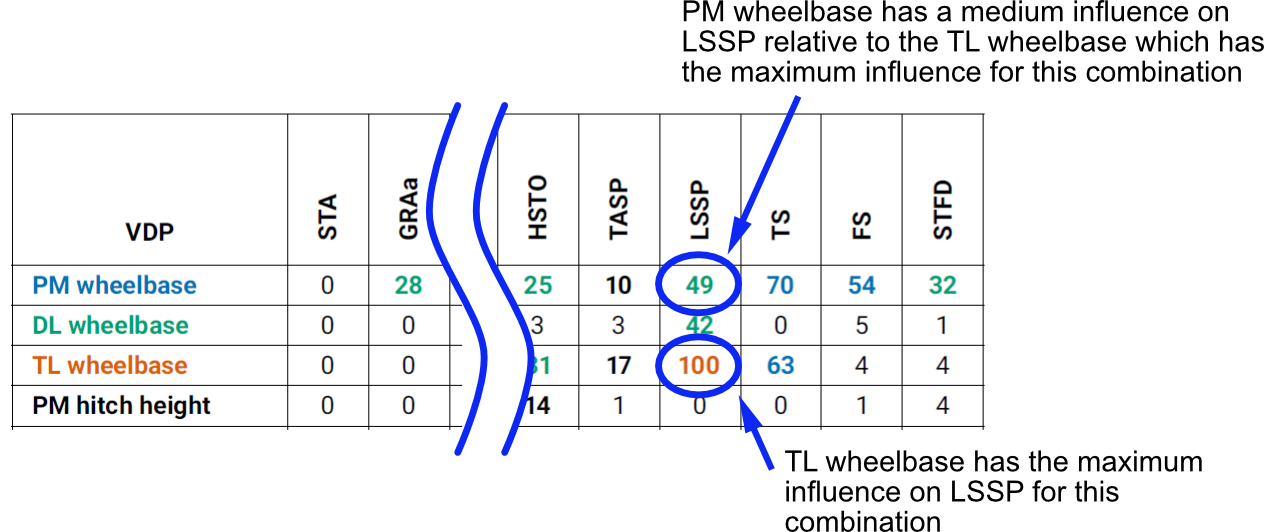
\includegraphics[width=1\textwidth]{fig/interpretation-of-cv-matrix}
        \caption{Interpretation of the \gls{cv} matrix}
        \label{figure:interpretation-of-cv-matrix}
    \end{figure}
%----------------------------------------------
%      FIGURE
%----------------------------------------------

To enhance the readability of the \gls{cv} matrices, the conventions and abbreviations detailed in Tables~\ref{table:cv-matrix-abbreviations}~to~\ref{table:cv-matrix-conventions} have been used throughout.

%----------------------------------------------
%      TABLE
%----------------------------------------------
\begin{table}[H]
	\centering\footnotesize
	\begin{threeparttable}

		\begin{tabulary}{\textwidth}{cl}
			\toprule
            
              \textbf{Abbreviation} & \textbf{Description}\\
              \midrule
              PM & Prime mover\\
              TL & Trailer\\
              St. & Steer axle\\
              Dr. & Drive axle\\
              Tl. & Trailer axle\\

			\bottomrule
		\end{tabulary}

		\caption{\gls{cv} matrix abbreviations}
		\label{table:cv-matrix-abbreviations}

		%\begin{tablenotes}
		%\item[1] %\tnote{1}
		%\end{tablenotes}

	\end{threeparttable}
\end{table}
%----------------------------------------------
%      TABLE
%----------------------------------------------

%-------------------------------------------------
%      TABLE

\begin{table}[H]
\centering\footnotesize
\begin{threeparttable}
\caption{CV matrix conventions}
\label{table:cv-matrix-conventions}

\begin{tabulary}{\textwidth}{ll}

\toprule
% Headings
\textbf{Format} & \textbf{Description}\\

\midrule
% Content
VDP Parameter 											     & \gls{vdp} without a relative influence above 10\% for any performance measure\\
\textbf{VDP Parameter}									     & \textbf{\gls{vdp} with a relative influence $\geq$ 10\% for at least 1 performance measure}\\
\textcolor[rgb]{0.000, 0.620, 0.451}{\textbf{VDP Parameter}} & \textcolor[rgb]{0.000, 0.620, 0.451}{\textbf{\gls{vdp} with a relative influence $\geq$ 25\% for at least 1 performance measure}}\\
\textcolor[rgb]{0.000, 0.447, 0.698}{\textbf{VDP Parameter}} & \textcolor[rgb]{0.000, 0.447, 0.698}{\textbf{\gls{vdp} with a relative influence $\geq$ 50\% for at least 1 performance measure}}\\
\textcolor[rgb]{0.835, 0.369, 0.000}{\textbf{VDP Parameter}} & \textcolor[rgb]{0.835, 0.369, 0.000}{\textbf{\gls{vdp} with a relative influence equal to 100\% for at least 1 performance measure}}\\
\midrule
5											       & \multicolumn{1}{l}{$0 \geq CV_n < 10$: \gls{vdp} has a negligible relative influence on the performance measure}\\
\textbf{15}										   & \multicolumn{1}{l}{\textbf{\textbf{$10 \geq CV_n < 25$: \gls{vdp} has a low relative influence on the performance measure}}}\\
\textcolor[rgb]{0.000, 0.620, 0.451}{\textbf{35}}  & \multicolumn{1}{l}{\textcolor[rgb]{0.000, 0.620, 0.451}{\textbf{$25 \geq CV_n < 50$: \gls{vdp} has a medium relative influence on the performance measure}}}\\
\textcolor[rgb]{0.000, 0.447, 0.698}{\textbf{65}}  & \multicolumn{1}{l}{\textcolor[rgb]{0.000, 0.447, 0.698}{\textbf{$50 \geq CV_n < 100$: \gls{vdp} has a high relative influence on the performance measure}}}\\
\textcolor[rgb]{0.835, 0.369, 0.000}{\textbf{100}} & \multicolumn{1}{l}{\textcolor[rgb]{0.835, 0.369, 0.000}{\textbf{$CV_n = 100 (CV_{max})$: \gls{vdp} has the maximum relative influence on the performance measure}}}\\
\bottomrule
\end{tabulary}

%\begin{tablenotes}
%\item[1] %\tnote{1}
%\end{tablenotes}

\end{threeparttable}
\end{table}

%      TABLE
%-------------------------------------------------

%==============================================
%      SECTION
%==============================================
\section{Overall CV Matrices}\label{sec:results-overall}

The overall \gls{cv} matrix for each of the baseline combinations is included in Tables~\ref{table:overall-cv-quad-semi}~to~\ref{table:overall-cv-rigid}. Only \glspl{vdp} with a relative influence of at least 10\% have been shown in these matrices to highlight the most influential parameters. A full \gls{cv} matrix with all evaluated parameters is included for each of the combinations in Appendix~\ref{appendix:complete-cv-matrix}.

%----------------------------------------------
%      TABLE

\begin{table}[H]

\centering\scriptsize

\caption{Overall \gls{cv} matrix - quad semi-trailer}
\label{table:overall-cv-quad-semi}

\begin{tabular}{|l|c|c|c|c|c|c|c|c|c|c|c|c|c|c|c|}
% Headings
\hline
\multicolumn{1}{|c|}{\textbf{VDP}} & \begin{sideways}\textbf{STA}\end{sideways} & \begin{sideways}\textbf{GRAa}\end{sideways} & \begin{sideways}\textbf{GRAb~~~~}\end{sideways} & \begin{sideways}\textbf{ACC}\end{sideways} & \begin{sideways}\textbf{SRTt}\end{sideways} & \begin{sideways}\textbf{YDC}\end{sideways} & \begin{sideways}\textbf{RA}\end{sideways} & \begin{sideways}\textbf{HSTO}\end{sideways} & \begin{sideways}\textbf{TASP}\end{sideways} & \begin{sideways}\textbf{LSSP}\end{sideways} & \begin{sideways}\textbf{TS}\end{sideways} & \begin{sideways}\textbf{FS}\end{sideways} & \begin{sideways}\textbf{MoD}\end{sideways} & \begin{sideways}\textbf{DoM}\end{sideways} & \begin{sideways}\textbf{STFD}\end{sideways} \bigstrut\\
% Contents
\hline
\textcolor[rgb]{0.851, 0.373, 0.008}{\textbf{PM wheelbase}} & 0 & \textcolor[rgb]{0.000, 0.447, 0.698}{\textbf{63}} & 0 & 0 & 3 & \textcolor[rgb]{0.000, 0.620, 0.451}{\textbf{40}} & \textbf{14} & \textcolor[rgb]{0.000, 0.447, 0.698}{\textbf{62}} & 4 & \textcolor[rgb]{0.000, 0.620, 0.451}{\textbf{31}} & 4 & \textcolor[rgb]{0.000, 0.447, 0.698}{\textbf{63}} & \textbf{16} & \textbf{19} & \textcolor[rgb]{0.835, 0.369, 0.000}{\textbf{100}} \\
\hline
\textcolor[rgb]{0.851, 0.373, 0.008}{\textbf{TL wheelbase}} & \textcolor[rgb]{0.835, 0.369, 0.000}{\textbf{100}} & \textcolor[rgb]{0.835, 0.369, 0.000}{\textbf{100}} & 0 & 0 & \textbf{18} & \textcolor[rgb]{0.000, 0.447, 0.698}{\textbf{70}} & \textcolor[rgb]{0.835, 0.369, 0.000}{\textbf{100}} & \textcolor[rgb]{0.000, 0.447, 0.698}{\textbf{80}} & 8 & \textcolor[rgb]{0.835, 0.369, 0.000}{\textbf{100}} & \textcolor[rgb]{0.000, 0.620, 0.451}{\textbf{44}} & 9 & 5 & 1 & 2 \\
\hline
\textbf{PM axle spacing} & 0 & 0 & 0 & 0 & 1 & 0 & 2 & 0 & 0 & 1 & 0 & 2 & 0 & 0 & \textbf{14} \\
\hline
\textbf{TL axle spacing} & 0 & 0 & 0 & 0 & 1 & 1 & 0 & \textbf{12} & 0 & 9 & 3 & 5 & 4 & 2 & 8 \\
\hline
\textcolor[rgb]{0.000, 0.620, 0.451}{\textbf{PM hitch long. loc.}} & 0 & \textcolor[rgb]{0.000, 0.620, 0.451}{\textbf{35}} & 0 & 0 & 1 & 9 & \textbf{12} & \textcolor[rgb]{0.000, 0.620, 0.451}{\textbf{33}} & 0 & 1 & 0 & 3 & 1 & 1 & \textbf{24} \\
\hline
\textbf{PM sprung mass} & \textbf{13} & 2 & 6 & 5 & 1 & 1 & 5 & 1 & 1 & 0 & 0 & 1 & 0 & 0 & \textbf{15} \\
\hline
\textcolor[rgb]{0.000, 0.620, 0.451}{\textbf{TL sprung mass}} & \textcolor[rgb]{0.000, 0.620, 0.451}{\textbf{48}} & 0 & \textbf{22} & \textbf{20} & 9 & 8 & \textbf{14} & 5 & 5 & 0 & 0 & 0 & 1 & 0 & 5 \\
\hline
\textbf{PM \gls{cgx}} & 0 & \textbf{10} & 0 & 0 & 0 & 0 & 5 & 3 & 0 & 0 & 0 & 0 & 0 & 0 & 7 \\
\hline
\textcolor[rgb]{0.000, 0.447, 0.698}{\textbf{TL \gls{cgx}}} & 0 & \textcolor[rgb]{0.000, 0.620, 0.451}{\textbf{49}} & 0 & 0 & \textbf{12} & 6 & \textcolor[rgb]{0.000, 0.447, 0.698}{\textbf{55}} & 8 & 2 & 1 & 0 & 2 & 1 & 1 & 2 \\
\hline
\textbf{TL \gls{cgy}} & 0 & 0 & 0 & 0 & \textbf{14} & 1 & 0 & 0 & \textbf{11} & 0 & 3 & 0 & 4 & 2 & 0 \\
\hline
\textbf{TL \gls{cgz}} & 0 & 0 & 0 & 0 & \textbf{22} & 1 & \textbf{22} & 3 & 2 & 0 & 0 & 0 & 0 & 0 & 0 \\
\hline
\textcolor[rgb]{0.000, 0.620, 0.451}{\textbf{TL \gls{iyy}/\gls{izz}}} & 0 & 0 & 0 & 0 & 1 & \textbf{19} & 5 & \textcolor[rgb]{0.000, 0.620, 0.451}{\textbf{38}} & 1 & 0 & 0 & 0 & 0 & 0 & 0 \\
\hline
\textcolor[rgb]{0.000, 0.447, 0.698}{\textbf{PM front overhang}} & 0 & 0 & 0 & 0 & 0 & 0 & 0 & 0 & 3 & \textbf{17} & 0 & \textcolor[rgb]{0.000, 0.447, 0.698}{\textbf{88}} & 3 & \textbf{11} & 0 \\
\hline
\textcolor[rgb]{0.851, 0.373, 0.008}{\textbf{TL front overhang}} & 0 & 0 & 0 & 0 & 0 & 0 & 0 & 0 & 0 & 0 & 0 & 0 & \textcolor[rgb]{0.835, 0.369, 0.000}{\textbf{100}} & \textcolor[rgb]{0.835, 0.369, 0.000}{\textbf{100}} & 0 \\
\hline
\textcolor[rgb]{0.851, 0.373, 0.008}{\textbf{TL rear overhang}} & 0 & 0 & 0 & 0 & 0 & 0 & 0 & 0 & \textcolor[rgb]{0.000, 0.620, 0.451}{\textbf{30}} & 0 & \textcolor[rgb]{0.835, 0.369, 0.000}{\textbf{100}} & 0 & 0 & 0 & 0 \\
\hline
\textcolor[rgb]{0.000, 0.447, 0.698}{\textbf{PM reference height}} & 0 & 0 & 0 & 0 & 0 & 0 & 0 & 0 & \textcolor[rgb]{0.000, 0.447, 0.698}{\textbf{76}} & 4 & 0 & \textbf{23} & 3 & 4 & 0 \\
\hline
\textcolor[rgb]{0.851, 0.373, 0.008}{\textbf{TL reference height}} & 0 & 0 & 0 & 0 & 0 & 0 & 0 & 0 & \textcolor[rgb]{0.835, 0.369, 0.000}{\textbf{100}} & 0 & 0 & 0 & 0 & 0 & 0 \\
\hline
\textcolor[rgb]{0.851, 0.373, 0.008}{\textbf{PM vehicle width}} & 0 & 0 & 0 & 0 & 0 & 0 & 0 & 0 & \textcolor[rgb]{0.000, 0.447, 0.698}{\textbf{77}} & \textbf{15} & 0 & \textcolor[rgb]{0.835, 0.369, 0.000}{\textbf{100}} & \textcolor[rgb]{0.000, 0.620, 0.451}{\textbf{37}} & \textbf{22} & 0 \\
\hline
\textcolor[rgb]{0.000, 0.447, 0.698}{\textbf{TL vehicle width}} & 0 & 0 & 0 & 0 & 0 & 0 & 0 & 0 & \textcolor[rgb]{0.000, 0.447, 0.698}{\textbf{59}} & 0 & \textbf{17} & 0 & \textcolor[rgb]{0.000, 0.620, 0.451}{\textbf{25}} & 6 & 0 \\
\hline
\textcolor[rgb]{0.851, 0.373, 0.008}{\textbf{TL payload mass}} & \textcolor[rgb]{0.000, 0.447, 0.698}{\textbf{56}} & 7 & \textcolor[rgb]{0.835, 0.369, 0.000}{\textbf{100}} & \textcolor[rgb]{0.835, 0.369, 0.000}{\textbf{100}} & \textcolor[rgb]{0.000, 0.620, 0.451}{\textbf{48}} & \textcolor[rgb]{0.835, 0.369, 0.000}{\textbf{100}} & \textcolor[rgb]{0.000, 0.447, 0.698}{\textbf{82}} & \textbf{20} & \textbf{21} & 2 & 2 & 3 & 4 & 3 & \textbf{22} \\
\hline
\textcolor[rgb]{0.000, 0.447, 0.698}{\textbf{TL payload \gls{cgx}}} & 0 & \textcolor[rgb]{0.000, 0.447, 0.698}{\textbf{57}} & 0 & 0 & \textbf{12} & 7 & \textbf{23} & 7 & 2 & 1 & 0 & 2 & 1 & 1 & 2 \\
\hline
\textcolor[rgb]{0.000, 0.620, 0.451}{\textbf{TL payload \gls{cgy}}} & 0 & 0 & 0 & 0 & \textcolor[rgb]{0.000, 0.620, 0.451}{\textbf{44}} & 4 & \textcolor[rgb]{0.000, 0.620, 0.451}{\textbf{26}} & 0 & \textcolor[rgb]{0.000, 0.620, 0.451}{\textbf{33}} & 0 & 8 & 1 & \textbf{11} & 6 & 0 \\
\hline
\textcolor[rgb]{0.851, 0.373, 0.008}{\textbf{TL payload \gls{cgz}}} & 0 & 0 & 0 & 0 & \textcolor[rgb]{0.835, 0.369, 0.000}{\textbf{100}} & 7 & 7 & \textbf{20} & \textbf{14} & 0 & 1 & 0 & 0 & 0 & 0 \\
\hline
\textcolor[rgb]{0.851, 0.373, 0.008}{\textbf{TL payload \gls{iyy}/\gls{izz}}} & 0 & 0 & 0 & 0 & 1 & \textcolor[rgb]{0.000, 0.447, 0.698}{\textbf{58}} & \textbf{18} & \textcolor[rgb]{0.835, 0.369, 0.000}{\textbf{100}} & 2 & 0 & 1 & 1 & 1 & 0 & 1 \\
\hline
\textcolor[rgb]{0.000, 0.447, 0.698}{\textbf{St. axle track}} & 0 & 0 & 0 & 0 & 0 & 0 & 0 & 0 & 0 & 4 & 1 & \textcolor[rgb]{0.000, 0.447, 0.698}{\textbf{79}} & 0 & 1 & 3 \\
\hline
\textbf{Tl. axle track} & 0 & 0 & 0 & 0 & \textbf{16} & 1 & 2 & 1 & 5 & 0 & 0 & 0 & 0 & 0 & 0 \\
\hline
\textbf{Dr. roll centre height} & 0 & 0 & 0 & 0 & 8 & 3 & \textbf{13} & 9 & 1 & 0 & 0 & 1 & 0 & 0 & 1 \\
\hline
\textbf{Dr. roll steer coef.} & 0 & 0 & 0 & 0 & 2 & \textbf{11} & 0 & 7 & 3 & 0 & 0 & 0 & 0 & 0 & 1 \\
\hline
\textbf{Tl. roll steer coef.} & 0 & 0 & 0 & 0 & 0 & 2 & 7 & \textbf{17} & \textbf{10} & 0 & 0 & 0 & 0 & 0 & 0 \\
\hline
\textbf{Dr. aux. roll stiffness} & 0 & 0 & 0 & 0 & \textbf{19} & 2 & \textbf{10} & 3 & 3 & 0 & 0 & 1 & 0 & 0 & 1 \\
\hline
\textcolor[rgb]{0.000, 0.620, 0.451}{\textbf{Tl. aux. roll stiffness}} & 0 & 0 & 0 & 0 & 7 & \textbf{11} & \textbf{11} & 9 & \textcolor[rgb]{0.000, 0.620, 0.451}{\textbf{35}} & 0 & 1 & 0 & 0 & 0 & 0 \\
\hline
\textbf{Dr. eff. rolling radius} & \textbf{15} & 0 & 1 & 3 & 0 & 0 & 0 & 0 & 0 & 0 & 0 & 0 & 0 & 0 & 0 \\
\hline
\textbf{Tl. tyre \gls{lagfymz}} & 0 & 0 & 0 & 0 & 2 & 4 & \textbf{14} & \textbf{14} & 0 & 0 & 0 & 0 & 0 & 0 & 0 \\
\hline
\textcolor[rgb]{0.000, 0.447, 0.698}{\textbf{St. cornering stiffness}} & 0 & 0 & 0 & 0 & 1 & \textcolor[rgb]{0.000, 0.447, 0.698}{\textbf{65}} & 2 & 2 & 1 & 0 & 0 & 0 & 0 & 0 & 7 \\
\hline
\textcolor[rgb]{0.000, 0.620, 0.451}{\textbf{Dr. cornering stiffness}} & 0 & 0 & 0 & 0 & 2 & 1 & \textcolor[rgb]{0.000, 0.620, 0.451}{\textbf{31}} & \textcolor[rgb]{0.000, 0.620, 0.451}{\textbf{49}} & 6 & 1 & 0 & 3 & 2 & 1 & \textbf{21} \\
\hline
\textcolor[rgb]{0.000, 0.447, 0.698}{\textbf{Tl. cornering stiffness}} & 0 & 0 & 0 & 0 & 1 & \textbf{10} & \textcolor[rgb]{0.000, 0.620, 0.451}{\textbf{33}} & \textcolor[rgb]{0.000, 0.447, 0.698}{\textbf{81}} & \textbf{23} & 1 & 0 & 2 & 2 & 1 & 3 \\
\hline

\end{tabular}%
\end{table}%

%      TABLE
%----------------------------------------------

%-------------------------------------------------
% 		LONG TABLE

\stdlongtable{
% Caption
Overall \gls{cv} matrix - tridem interlink
}{
% Label
\label{table:overall-cv-tridem-interlink}
}{
% Column specification
|l|c|c|c|c|c|c|c|c|c|c|c|c|c|c|c|
}{
% Headings
\multicolumn{1}{|c|}{\textbf{VDP}} & \begin{sideways}\textbf{STA}\end{sideways} & \begin{sideways}\textbf{GRAa}\end{sideways} & \begin{sideways}\textbf{GRAb~~~~}\end{sideways} & \begin{sideways}\textbf{ACC}\end{sideways} & \begin{sideways}\textbf{SRTt}\end{sideways} & \begin{sideways}\textbf{YDC}\end{sideways} & \begin{sideways}\textbf{RA}\end{sideways} & \begin{sideways}\textbf{HSTO}\end{sideways} & \begin{sideways}\textbf{TASP}\end{sideways} & \begin{sideways}\textbf{LSSP}\end{sideways} & \begin{sideways}\textbf{TS}\end{sideways} & \begin{sideways}\textbf{FS}\end{sideways} & \begin{sideways}\textbf{MoD}\end{sideways} & \begin{sideways}\textbf{DoM}\end{sideways} & \begin{sideways}\textbf{STFD}\end{sideways} \bigstrut

}{
% Width
1\textwidth
}{
% portrait/landscape
portrait
}{
% fontspec
\scriptsize
}{
% Contents
    \hline
    \textcolor[rgb]{0.851, 0.373, 0.008}{\textbf{PM wheelbase}} & 0 & \textcolor[rgb]{0.000, 0.620, 0.451}{\textbf{43}} & 0 & 0 & 3 & \textbf{16} & \textbf{20} & \textcolor[rgb]{0.000, 0.447, 0.698}{\textbf{62}} & 5 & \textcolor[rgb]{0.000, 0.620, 0.451}{\textbf{43}} & \textbf{21} & \textcolor[rgb]{0.000, 0.447, 0.698}{\textbf{62}} & \textbf{24} & 4 & \textcolor[rgb]{0.835, 0.369, 0.000}{\textbf{100}} \\
    \hline
    \textcolor[rgb]{0.000, 0.620, 0.451}{\textbf{TL 1 wheelbase}} & 0 & \textbf{11} & 0 & 0 & 4 & 8 & 7 & \textbf{17} & 0 & \textcolor[rgb]{0.000, 0.620, 0.451}{\textbf{34}} & 5 & 1 & 5 & 0 & 0 \\
    \hline
    \textcolor[rgb]{0.851, 0.373, 0.008}{\textbf{TL 2 wheelbase}} & 0 & 8 & 0 & 0 & \textbf{11} & \textcolor[rgb]{0.835, 0.369, 0.000}{\textbf{100}} & \textbf{19} & \textcolor[rgb]{0.835, 0.369, 0.000}{\textbf{100}} & \textcolor[rgb]{0.000, 0.620, 0.451}{\textbf{40}} & \textcolor[rgb]{0.835, 0.369, 0.000}{\textbf{100}} & \textcolor[rgb]{0.000, 0.620, 0.451}{\textbf{42}} & 4 & 8 & 0 & 4 \\
    \hline
    \textbf{PM axle spacing} & 0 & 0 & 0 & 0 & 0 & 1 & 0 & 0 & 0 & 1 & 0 & 2 & 1 & 0 & \textbf{13} \\
    \hline
    \textbf{TL 2 axle spacing} & 0 & 0 & 0 & 0 & 0 & 0 & 1 & \textbf{10} & 0 & 3 & \textbf{10} & 1 & 4 & 0 & 1 \\
    \hline
    \textcolor[rgb]{0.000, 0.620, 0.451}{\textbf{PM hitch long. loc.}} & 0 & \textbf{21} & 0 & 0 & 1 & \textbf{12} & 6 & \textcolor[rgb]{0.000, 0.620, 0.451}{\textbf{25}} & 1 & 1 & 1 & 3 & 0 & 0 & \textcolor[rgb]{0.000, 0.620, 0.451}{\textbf{25}} \\
    \hline
    \textbf{TL 1 hitch long. loc.} & 0 & 6 & 0 & 0 & 2 & 1 & 7 & \textbf{16} & 4 & 6 & 6 & 0 & 1 & 0 & 1 \\
    \hline
    \textbf{PM sprung mass} & 5 & 1 & 9 & 8 & 2 & 3 & 1 & 0 & 1 & 0 & 1 & 0 & 0 & 0 & \textbf{19} \\
    \hline
    \textbf{TL 1 sprung mass} & 6 & 5 & \textbf{12} & \textbf{10} & 2 & 1 & 0 & 4 & 2 & 0 & 0 & 0 & 0 & 0 & 1 \\
    \hline
    \textbf{TL 2 sprung mass} & 6 & 6 & \textbf{11} & \textbf{10} & 6 & 9 & 7 & 0 & 2 & 0 & 0 & 0 & 0 & 0 & 0 \\
    \hline
    \textcolor[rgb]{0.000, 0.620, 0.451}{\textbf{TL 1 \gls{cgx}}} & 0 & \textbf{10} & 0 & 0 & 4 & 1 & \textcolor[rgb]{0.000, 0.620, 0.451}{\textbf{39}} & 3 & 0 & 0 & 0 & 1 & 1 & 0 & 1 \\
    \hline
    \textbf{PM \gls{cgy}} & 0 & 0 & 0 & 0 & 7 & 3 & 6 & 2 & 4 & 1 & \textbf{10} & 1 & 2 & 0 & 1 \\
    \hline
    \textbf{TL 1 \gls{cgy}} & 0 & 0 & 0 & 0 & \textbf{11} & 1 & 7 & 1 & 3 & 1 & 6 & 0 & 2 & 0 & 0 \\
    \hline
    \textbf{TL 2 \gls{cgy}} & 0 & 0 & 0 & 0 & \textbf{17} & 0 & 8 & 2 & 5 & 0 & 9 & 0 & 0 & 0 & 0 \\
    \hline
    \textbf{TL 1 \gls{cgz}} & 0 & 0 & 0 & 0 & \textbf{11} & 0 & 3 & 2 & 0 & 0 & 0 & 0 & 0 & 0 & 0 \\
    \hline
    \textbf{TL 2 \gls{cgz}} & 0 & 0 & 0 & 0 & \textbf{19} & 1 & \textbf{10} & 2 & 1 & 0 & 0 & 0 & 0 & 0 & 0 \\
    \hline
    \textbf{PM \gls{ixx}} & 0 & 0 & 0 & 0 & 0 & 0 & \textbf{14} & 0 & 0 & 0 & 0 & 0 & 0 & 0 & 0 \\
    \hline
    \textbf{TL 2 \gls{iyy}/\gls{izz}} & 0 & 0 & 0 & 0 & 0 & \textbf{14} & 7 & \textbf{15} & 0 & 0 & 0 & 0 & 0 & 0 & 0 \\
    \hline
    \textcolor[rgb]{0.000, 0.447, 0.698}{\textbf{PM front overhang}} & 0 & 0 & 0 & 0 & 0 & 0 & 0 & 0 & 2 & \textcolor[rgb]{0.000, 0.620, 0.451}{\textbf{25}} & 0 & \textcolor[rgb]{0.000, 0.447, 0.698}{\textbf{89}} & 6 & 1 & 0 \\
    \hline
    \textcolor[rgb]{0.851, 0.373, 0.008}{\textbf{TL 1 front overhang}} & 0 & 0 & 0 & 0 & 0 & 0 & 0 & 0 & 0 & 0 & 0 & 0 & \textcolor[rgb]{0.835, 0.369, 0.000}{\textbf{100}} & \textcolor[rgb]{0.835, 0.369, 0.000}{\textbf{100}} & 0 \\
    \hline
    \textcolor[rgb]{0.000, 0.447, 0.698}{\textbf{TL 2 rear overhang}} & 0 & 0 & 0 & 0 & 0 & 0 & 0 & 0 & \textbf{17} & 0 & \textcolor[rgb]{0.000, 0.447, 0.698}{\textbf{54}} & 0 & 0 & 0 & 0 \\
    \hline
    \textcolor[rgb]{0.000, 0.447, 0.698}{\textbf{PM reference height}} & 0 & 0 & 0 & 0 & 0 & 0 & 0 & 0 & \textcolor[rgb]{0.000, 0.447, 0.698}{\textbf{59}} & 6 & 0 & \textbf{24} & 4 & 0 & 0 \\
    \hline
    \textcolor[rgb]{0.000, 0.447, 0.698}{\textbf{TL 1 reference height}} & 0 & 0 & 0 & 0 & 0 & 0 & 0 & 0 & \textcolor[rgb]{0.000, 0.447, 0.698}{\textbf{95}} & 0 & 0 & 0 & 3 & 0 & 0 \\
    \hline
    \textcolor[rgb]{0.851, 0.373, 0.008}{\textbf{TL 2 reference height}} & 0 & 0 & 0 & 0 & 0 & 0 & 0 & 0 & \textcolor[rgb]{0.835, 0.369, 0.000}{\textbf{100}} & 0 & 0 & 0 & 0 & 0 & 0 \\
    \hline
    \textcolor[rgb]{0.851, 0.373, 0.008}{\textbf{PM vehicle width}} & 0 & 0 & 0 & 0 & 0 & 0 & 0 & 0 & \textcolor[rgb]{0.000, 0.447, 0.698}{\textbf{59}} & \textbf{22} & 0 & \textcolor[rgb]{0.835, 0.369, 0.000}{\textbf{100}} & \textcolor[rgb]{0.000, 0.447, 0.698}{\textbf{50}} & 4 & 0 \\
    \hline
    \textcolor[rgb]{0.000, 0.620, 0.451}{\textbf{TL 1 vehicle width}} & 0 & 0 & 0 & 0 & 0 & 0 & 0 & 0 & 0 & 0 & 0 & 0 & \textcolor[rgb]{0.000, 0.620, 0.451}{\textbf{38}} & 3 & 0 \\
    \hline
    \textcolor[rgb]{0.851, 0.373, 0.008}{\textbf{TL 2 vehicle width}} & 0 & 0 & 0 & 0 & 0 & 0 & 0 & 0 & \textcolor[rgb]{0.000, 0.620, 0.451}{\textbf{45}} & 0 & \textcolor[rgb]{0.835, 0.369, 0.000}{\textbf{100}} & 0 & 0 & 0 & 0 \\
    \hline
    \textcolor[rgb]{0.851, 0.373, 0.008}{\textbf{TL 1 payload mass}} & \textcolor[rgb]{0.835, 0.369, 0.000}{\textbf{100}} & \textcolor[rgb]{0.835, 0.369, 0.000}{\textbf{100}} & \textcolor[rgb]{0.835, 0.369, 0.000}{\textbf{100}} & \textcolor[rgb]{0.835, 0.369, 0.000}{\textbf{100}} & \textcolor[rgb]{0.835, 0.369, 0.000}{\textbf{100}} & \textcolor[rgb]{0.000, 0.620, 0.451}{\textbf{40}} & \textcolor[rgb]{0.000, 0.620, 0.451}{\textbf{47}} & \textcolor[rgb]{0.000, 0.620, 0.451}{\textbf{36}} & \textbf{15} & \textbf{11} & 2 & 4 & 5 & 1 & \textbf{20} \\
    \hline
    \textcolor[rgb]{0.851, 0.373, 0.008}{\textbf{TL 2 payload mass}} & \textcolor[rgb]{0.000, 0.447, 0.698}{\textbf{67}} & \textcolor[rgb]{0.000, 0.447, 0.698}{\textbf{59}} & \textcolor[rgb]{0.835, 0.369, 0.000}{\textbf{100}} & \textcolor[rgb]{0.835, 0.369, 0.000}{\textbf{100}} & \textbf{13} & \textcolor[rgb]{0.000, 0.620, 0.451}{\textbf{27}} & 6 & \textcolor[rgb]{0.000, 0.620, 0.451}{\textbf{25}} & \textbf{20} & 6 & 2 & 1 & 1 & 0 & 1 \\
    \hline
    \textbf{TL 1 payload \gls{cgx}} & 0 & \textbf{18} & 0 & 0 & 9 & 0 & \textbf{12} & 6 & 1 & 0 & 0 & 1 & 1 & 0 & 1 \\
    \hline
    \textbf{TL 2 payload \gls{cgx}} & 0 & 3 & 0 & 0 & \textbf{11} & \textbf{11} & \textbf{13} & 9 & 0 & 1 & 0 & 1 & 2 & 0 & 1 \\
    \hline
    \textcolor[rgb]{0.000, 0.447, 0.698}{\textbf{TL 1 payload \gls{cgy}}} & 0 & 0 & 0 & 0 & \textcolor[rgb]{0.000, 0.447, 0.698}{\textbf{75}} & 1 & 8 & 4 & \textbf{16} & 4 & \textcolor[rgb]{0.000, 0.620, 0.451}{\textbf{26}} & 1 & 9 & 1 & 0 \\
    \hline
    \textcolor[rgb]{0.000, 0.447, 0.698}{\textbf{TL 2 payload \gls{cgy}}} & 0 & 0 & 0 & 0 & \textcolor[rgb]{0.000, 0.447, 0.698}{\textbf{94}} & 0 & \textbf{24} & \textbf{12} & \textcolor[rgb]{0.000, 0.620, 0.451}{\textbf{29}} & 2 & \textcolor[rgb]{0.000, 0.620, 0.451}{\textbf{28}} & 0 & 2 & 1 & 0 \\
    \hline
    \textcolor[rgb]{0.000, 0.447, 0.698}{\textbf{TL 1 payload \gls{cgz}}} & 0 & 0 & 0 & 0 & \textcolor[rgb]{0.000, 0.447, 0.698}{\textbf{75}} & 7 & \textbf{13} & 9 & 2 & 0 & 1 & 0 & 0 & 0 & 0 \\
    \hline
    \textcolor[rgb]{0.000, 0.447, 0.698}{\textbf{TL 2 payload \gls{cgz}}} & 0 & 0 & 0 & 0 & \textcolor[rgb]{0.000, 0.447, 0.698}{\textbf{95}} & 6 & 9 & \textbf{15} & 9 & 0 & 1 & 0 & 0 & 0 & 0 \\
    \hline
    \textbf{TL 1 payload \gls{ixx}} & 0 & 0 & 0 & 0 & 1 & 0 & \textbf{14} & 0 & 0 & 0 & 0 & 0 & 0 & 0 & 0 \\
    \hline
    \textbf{TL 2 payload \gls{ixx}} & 0 & 0 & 0 & 0 & 1 & 1 & \textbf{14} & 2 & 1 & 0 & 0 & 0 & 0 & 0 & 0 \\
    \hline
    \textbf{TL 1 payload \gls{iyy}/\gls{izz}} & 0 & 0 & 0 & 0 & 0 & 8 & 8 & \textbf{22} & 1 & 0 & 1 & 0 & 0 & 0 & 0 \\
    \hline
    \textcolor[rgb]{0.000, 0.620, 0.451}{\textbf{TL 2 payload \gls{iyy}/\gls{izz}}} & 0 & 0 & 0 & 0 & 1 & \textcolor[rgb]{0.000, 0.620, 0.451}{\textbf{43}} & \textbf{17} & \textcolor[rgb]{0.000, 0.620, 0.451}{\textbf{49}} & 1 & 0 & 1 & 0 & 0 & 0 & 0 \\
    \hline
    \textbf{Tl. unsprung mass} & 5 & 4 & 8 & 7 & \textbf{16} & 1 & 1 & 2 & 1 & 0 & 0 & 0 & 0 & 0 & 0 \\
    \hline
    \textcolor[rgb]{0.000, 0.447, 0.698}{\textbf{St. axle track}} & 0 & 0 & 0 & 0 & 0 & 0 & 0 & 0 & 0 & 5 & \textbf{17} & \textcolor[rgb]{0.000, 0.447, 0.698}{\textbf{79}} & 0 & 0 & 3 \\
    \hline
    \textcolor[rgb]{0.000, 0.620, 0.451}{\textbf{Tl. axle track}} & 0 & 0 & 0 & 0 & \textcolor[rgb]{0.000, 0.620, 0.451}{\textbf{44}} & 1 & 4 & 4 & 4 & 0 & 0 & 0 & 0 & 0 & 0 \\
    \hline
    \textcolor[rgb]{0.000, 0.620, 0.451}{\textbf{Dr. roll centre height}} & 0 & 0 & 0 & 0 & \textbf{12} & 0 & 2 & 6 & 1 & 1 & 0 & 1 & 1 & 0 & \textcolor[rgb]{0.000, 0.620, 0.451}{\textbf{36}} \\
    \hline
    \textbf{Tl. roll steer coef.} & 0 & 0 & 0 & 0 & 0 & 4 & 1 & \textbf{21} & \textbf{18} & 0 & 0 & 0 & 0 & 0 & 0 \\
    \hline
    \textbf{Dr. spin inertia} & 0 & 0 & 0 & 0 & 0 & 0 & 0 & 0 & 0 & 1 & 0 & 1 & 1 & 0 & \textbf{22} \\
    \hline
    \textcolor[rgb]{0.000, 0.620, 0.451}{\textbf{Dr. aux. roll stiffness}} & 0 & 0 & 0 & 0 & \textcolor[rgb]{0.000, 0.620, 0.451}{\textbf{25}} & 2 & 8 & 1 & 2 & 0 & 1 & 1 & 0 & 0 & 1 \\
    \hline
    \textcolor[rgb]{0.851, 0.373, 0.008}{\textbf{Tl. aux. roll stiffness}} & 0 & 0 & 0 & 0 & \textcolor[rgb]{0.000, 0.620, 0.451}{\textbf{47}} & \textbf{17} & \textcolor[rgb]{0.835, 0.369, 0.000}{\textbf{100}} & \textbf{14} & \textcolor[rgb]{0.000, 0.447, 0.698}{\textbf{99}} & 0 & 9 & 0 & 1 & 0 & 0 \\
    \hline
    \textbf{Tl. tyre \gls{lagfymz}} & 0 & 0 & 0 & 0 & 2 & 7 & \textbf{11} & \textbf{21} & 2 & 0 & 2 & 0 & 1 & 0 & 0 \\
    \hline
    \textbf{St. cornering stiffness} & 0 & 0 & 0 & 0 & 0 & \textbf{19} & 3 & 1 & 2 & 0 & 0 & 0 & 0 & 0 & 6 \\
    \hline
    \textcolor[rgb]{0.000, 0.620, 0.451}{\textbf{Dr. cornering stiffness}} & 0 & 0 & 0 & 0 & 0 & 5 & 6 & \textcolor[rgb]{0.000, 0.620, 0.451}{\textbf{32}} & 3 & 2 & 0 & 3 & 2 & 0 & \textbf{19} \\
    \hline
    \textcolor[rgb]{0.000, 0.447, 0.698}{\textbf{Tl. cornering stiffness}} & 0 & 0 & 0 & 0 & 1 & \textbf{13} & 6 & \textcolor[rgb]{0.000, 0.447, 0.698}{\textbf{94}} & \textbf{22} & 1 & 3 & 2 & 3 & 0 & 3 \\
    \hline
    \textbf{Tl. spring rate} & 0 & 0 & 0 & 0 & \textbf{13} & 6 & \textbf{22} & 2 & 3 & 0 & 0 & 0 & 0 & 0 & 0 \\
    \hline

}{16}

% 		LONG TABLE
%-------------------------------------------------
\newpage
%----------------------------------------------
%      LONG TABLE

\stdlongtable{
% Caption
Overall \gls{cv} matrix - rigid drawbar combination
}{
% Label
\label{table:overall-cv-rigid}
}{
% Column specification
|l|c|c|c|c|c|c|c|c|c|c|c|c|c|c|
}{
% Headings
\multicolumn{1}{|c|}{\textbf{VDP}} & \begin{sideways}\textbf{STA}\end{sideways} & \begin{sideways}\textbf{GRAa}\end{sideways} & \begin{sideways}\textbf{GRAb}\end{sideways} & \begin{sideways}\textbf{ACC}\end{sideways} & \begin{sideways}\textbf{SRTt}\end{sideways} & \begin{sideways}\textbf{SRTtrrcu~~~~}\end{sideways} & \begin{sideways}\textbf{YDC}\end{sideways} & \begin{sideways}\textbf{RA}\end{sideways} & \begin{sideways}\textbf{HSTO}\end{sideways} & \begin{sideways}\textbf{TASP}\end{sideways} & \begin{sideways}\textbf{LSSP}\end{sideways} & \begin{sideways}\textbf{TS}\end{sideways} & \begin{sideways}\textbf{FS}\end{sideways} & \begin{sideways}\textbf{STFD}\end{sideways} \bigstrut
}{
% Width
1\textwidth
}{
% portrait/landscape
portrait
}{
% fontspec
\scriptsize
}{
% Contents
\hline
\textcolor[rgb]{0.000, 0.447, 0.698}{\textbf{PM wheelbase}} & 0 & \textcolor[rgb]{0.000, 0.620, 0.451}{\textbf{28}} & 0 & 0 & 8 & 0 & \textcolor[rgb]{0.000, 0.620, 0.451}{\textbf{43}} & \textbf{21} & \textcolor[rgb]{0.000, 0.620, 0.451}{\textbf{25}} & \textbf{10} & \textcolor[rgb]{0.000, 0.620, 0.451}{\textbf{49}} & \textcolor[rgb]{0.000, 0.447, 0.698}{\textbf{70}} & \textcolor[rgb]{0.000, 0.447, 0.698}{\textbf{54}} & \textcolor[rgb]{0.000, 0.620, 0.451}{\textbf{32}} \\
\hline
\textcolor[rgb]{0.000, 0.620, 0.451}{\textbf{DL wheelbase}} & 0 & 0 & 0 & 0 & 1 & 0 & 2 & 4 & 3 & 3 & \textcolor[rgb]{0.000, 0.620, 0.451}{\textbf{42}} & 0 & 5 & 1 \\
\hline
\textcolor[rgb]{0.851, 0.373, 0.008}{\textbf{TL wheelbase}} & 0 & 0 & 0 & 0 & \textbf{17} & \textbf{12} & \textcolor[rgb]{0.000, 0.620, 0.451}{\textbf{44}} & \textcolor[rgb]{0.000, 0.447, 0.698}{\textbf{55}} & \textcolor[rgb]{0.000, 0.620, 0.451}{\textbf{31}} & \textbf{17} & \textcolor[rgb]{0.835, 0.369, 0.000}{\textbf{100}} & \textcolor[rgb]{0.000, 0.447, 0.698}{\textbf{63}} & 4 & 4 \\
\hline
\textbf{PM hitch height} & 0 & 0 & 0 & 0 & 1 & 0 & 2 & \textbf{14} & \textbf{14} & 1 & 0 & 0 & 1 & 4 \\
\hline
\textbf{PM hitch long. loc.} & 0 & 0 & 0 & 0 & 0 & 0 & 3 & \textbf{15} & \textbf{19} & 3 & \textbf{11} & 4 & 0 & 3 \\
\hline
\textbf{DL hitch long. loc.} & 0 & 0 & 0 & 0 & 3 & 2 & \textbf{18} & 6 & 4 & 2 & 3 & 1 & 1 & 4 \\
\hline
\textbf{PM sprung mass} & 3 & 1 & 6 & 4 & 0 & 0 & 3 & 1 & 1 & 0 & 1 & 1 & 1 & \textbf{18} \\
\hline
\textbf{PM \gls{cgy}} & 0 & 0 & 0 & 0 & \textbf{14} & 0 & 3 & 0 & 2 & 2 & 1 & 7 & 2 & 6 \\
\hline
\textcolor[rgb]{0.851, 0.373, 0.008}{\textbf{PM front overhang}} & 0 & 0 & 0 & 0 & 0 & 0 & 0 & 0 & 0 & 1 & \textbf{18} & 0 & \textcolor[rgb]{0.835, 0.369, 0.000}{\textbf{100}} & 0 \\
\hline
\textcolor[rgb]{0.000, 0.447, 0.698}{\textbf{PM rear overhang}} & 0 & 0 & 0 & 0 & 0 & 0 & 0 & 0 & 0 & 0 & 0 & \textcolor[rgb]{0.000, 0.447, 0.698}{\textbf{91}} & 0 & 0 \\
\hline
\textcolor[rgb]{0.851, 0.373, 0.008}{\textbf{TL rear overhang}} & 0 & 0 & 0 & 0 & 0 & 0 & 0 & 0 & 0 & \textbf{11} & 0 & \textcolor[rgb]{0.835, 0.369, 0.000}{\textbf{100}} & 0 & 0 \\
\hline
\textcolor[rgb]{0.000, 0.447, 0.698}{\textbf{PM reference height}} & 0 & 0 & 0 & 0 & 0 & 0 & 0 & 0 & 0 & \textcolor[rgb]{0.000, 0.447, 0.698}{\textbf{63}} & 4 & 9 & \textbf{23} & 0 \\
\hline
\textcolor[rgb]{0.000, 0.447, 0.698}{\textbf{TL reference height}} & 0 & 0 & 0 & 0 & 0 & 0 & 0 & 0 & 0 & \textcolor[rgb]{0.000, 0.447, 0.698}{\textbf{66}} & 0 & 0 & 0 & 0 \\
\hline
\textcolor[rgb]{0.000, 0.447, 0.698}{\textbf{PM vehicle width}} & 0 & 0 & 0 & 0 & 0 & 0 & 0 & 0 & 0 & \textcolor[rgb]{0.000, 0.447, 0.698}{\textbf{50}} & \textbf{13} & \textcolor[rgb]{0.000, 0.620, 0.451}{\textbf{49}} & \textcolor[rgb]{0.000, 0.447, 0.698}{\textbf{85}} & 0 \\
\hline
\textcolor[rgb]{0.000, 0.620, 0.451}{\textbf{TL vehicle width}} & 0 & 0 & 0 & 0 & 0 & 0 & 0 & 0 & 0 & \textcolor[rgb]{0.000, 0.620, 0.451}{\textbf{28}} & 0 & 0 & 0 & 0 \\
\hline
\textcolor[rgb]{0.851, 0.373, 0.008}{\textbf{PM payload mass}} & \textcolor[rgb]{0.835, 0.369, 0.000}{\textbf{100}} & \textcolor[rgb]{0.835, 0.369, 0.000}{\textbf{100}} & \textcolor[rgb]{0.000, 0.620, 0.451}{\textbf{45}} & \textcolor[rgb]{0.000, 0.620, 0.451}{\textbf{40}} & 0 & 0 & \textbf{19} & \textbf{17} & 9 & 8 & \textbf{16} & 4 & \textbf{17} & \textcolor[rgb]{0.000, 0.620, 0.451}{\textbf{31}} \\
\hline
\textcolor[rgb]{0.851, 0.373, 0.008}{\textbf{TL payload mass}} & \textcolor[rgb]{0.000, 0.447, 0.698}{\textbf{67}} & \textcolor[rgb]{0.000, 0.620, 0.451}{\textbf{36}} & \textcolor[rgb]{0.835, 0.369, 0.000}{\textbf{100}} & \textcolor[rgb]{0.835, 0.369, 0.000}{\textbf{100}} & \textbf{18} & \textcolor[rgb]{0.000, 0.447, 0.698}{\textbf{79}} & \textcolor[rgb]{0.835, 0.369, 0.000}{\textbf{100}} & \textcolor[rgb]{0.835, 0.369, 0.000}{\textbf{100}} & \textcolor[rgb]{0.000, 0.447, 0.698}{\textbf{65}} & \textbf{14} & 7 & 0 & 5 & 5 \\
\hline
\textbf{PM payload \gls{cgx}} & 0 & \textbf{12} & 0 & 0 & 3 & 0 & 7 & 3 & 1 & 3 & 3 & 1 & 2 & \textbf{22} \\
\hline
\textbf{TL payload \gls{cgx}} & 0 & 0 & 0 & 0 & \textbf{18} & 9 & 4 & 2 & 4 & 1 & 1 & 0 & 2 & 2 \\
\hline
\textcolor[rgb]{0.000, 0.447, 0.698}{\textbf{PM payload \gls{cgy}}} & 0 & 0 & 0 & 0 & \textcolor[rgb]{0.000, 0.447, 0.698}{\textbf{50}} & 0 & 4 & 1 & 4 & 4 & 1 & \textbf{14} & 4 & \textbf{10} \\
\hline
\textcolor[rgb]{0.000, 0.447, 0.698}{\textbf{TL payload \gls{cgy}}} & 0 & 0 & 0 & 0 & \textcolor[rgb]{0.000, 0.447, 0.698}{\textbf{85}} & \textcolor[rgb]{0.000, 0.620, 0.451}{\textbf{40}} & 2 & 5 & 9 & \textcolor[rgb]{0.000, 0.620, 0.451}{\textbf{30}} & 2 & \textcolor[rgb]{0.000, 0.620, 0.451}{\textbf{39}} & 0 & 0 \\
\hline
\textcolor[rgb]{0.000, 0.620, 0.451}{\textbf{PM payload \gls{cgz}}} & 0 & 0 & 0 & 0 & \textcolor[rgb]{0.000, 0.620, 0.451}{\textbf{43}} & 0 & 6 & \textcolor[rgb]{0.000, 0.620, 0.451}{\textbf{46}} & \textcolor[rgb]{0.000, 0.620, 0.451}{\textbf{26}} & 7 & 0 & 1 & 1 & 1 \\
\hline
\textcolor[rgb]{0.851, 0.373, 0.008}{\textbf{TL payload \gls{cgz}}} & 0 & 0 & 0 & 0 & \textcolor[rgb]{0.000, 0.447, 0.698}{\textbf{82}} & \textcolor[rgb]{0.835, 0.369, 0.000}{\textbf{100}} & \textcolor[rgb]{0.000, 0.620, 0.451}{\textbf{32}} & \textbf{23} & \textcolor[rgb]{0.000, 0.620, 0.451}{\textbf{30}} & \textbf{16} & 0 & 0 & 0 & 0 \\
\hline
\textcolor[rgb]{0.000, 0.620, 0.451}{\textbf{PM payload \gls{ixx}}} & 0 & 0 & 0 & 0 & 0 & 0 & \textbf{21} & \textcolor[rgb]{0.000, 0.620, 0.451}{\textbf{34}} & \textcolor[rgb]{0.000, 0.620, 0.451}{\textbf{38}} & \textbf{15} & 0 & 0 & 0 & 0\\
\hline
\textbf{TL payload \gls{iyy}/\gls{izz}} & 0 & 0 & 0 & 0 & 1 & 0 & \textbf{13} & 8 & \textbf{19} & 3 & 0 & 0 & 0 & 0 \\
\hline
\textbf{Tl. unsprung mass} & 3 & 3 & 5 & 4 & \textbf{10} & 5 & 0 & 1 & 1 & 0 & 0 & 0 & 0 & 1 \\
\hline
\textcolor[rgb]{0.000, 0.447, 0.698}{\textbf{St. axle track}} & 0 & 0 & 0 & 0 & 0 & 0 & 0 & 0 & 0 & 0 & 4 & 0 & \textcolor[rgb]{0.000, 0.447, 0.698}{\textbf{70}} & \textcolor[rgb]{0.000, 0.620, 0.451}{\textbf{35}} \\
\hline
\textcolor[rgb]{0.000, 0.620, 0.451}{\textbf{Tl. axle track}} & 0 & 0 & 0 & 0 & \textcolor[rgb]{0.000, 0.620, 0.451}{\textbf{36}} & \textbf{17} & 2 & 2 & 3 & 5 & 0 & 0 & 0 & 0 \\
\hline
\textbf{Dr. roll centre height} & 0 & 0 & 0 & 0 & 4 & 0 & 5 & \textbf{11} & 7 & 0 & 1 & 1 & 1 & 1 \\
\hline
\textbf{St. roll steer coef.} & 0 & 0 & 0 & 0 & 0 & 0 & \textbf{10} & 0 & 0 & 0 & 0 & 0 & 0 & 2 \\
\hline
\textbf{Dr. roll steer coef.} & 0 & 0 & 0 & 0 & 0 & 0 & \textcolor[rgb]{0.000, 0.620, 0.451}{\textbf{25}} & 8 & \textbf{21} & \textbf{12} & 0 & 2 & 1 & 1 \\
\hline
\textbf{Tl. roll steer coef.} & 0 & 0 & 0 & 0 & 0 & 1 & 3 & 0 & \textbf{15} & 6 & 0 & 0 & 0 & 0 \\
\hline
\textbf{Tl. spin inertia} & 0 & 0 & 0 & 0 & 5 & \textbf{13} & 0 & 0 & 0 & 0 & 0 & 0 & 0 & 0 \\
\hline
\textbf{St. aux. roll stiffness} & 0 & 0 & 0 & 0 & 8 & 0 & 1 & \textbf{11} & \textbf{11} & 3 & 0 & 0 & 0 & 1 \\
\hline
\textcolor[rgb]{0.851, 0.373, 0.008}{\textbf{Dr. aux. roll stiffness}} & 0 & 0 & 0 & 0 & \textcolor[rgb]{0.000, 0.447, 0.698}{\textbf{77}} & 0 & \textcolor[rgb]{0.000, 0.620, 0.451}{\textbf{46}} & \textcolor[rgb]{0.000, 0.447, 0.698}{\textbf{68}} & \textcolor[rgb]{0.835, 0.369, 0.000}{\textbf{100}} & 8 & 0 & 1 & 2 & 4 \\
\hline
\textcolor[rgb]{0.851, 0.373, 0.008}{\textbf{Tl. aux. roll stiffness}} & 0 & 0 & 0 & 0 & \textcolor[rgb]{0.835, 0.369, 0.000}{\textbf{100}} & \textcolor[rgb]{0.000, 0.620, 0.451}{\textbf{46}} & \textcolor[rgb]{0.000, 0.620, 0.451}{\textbf{28}} & \textcolor[rgb]{0.000, 0.447, 0.698}{\textbf{70}} & \textbf{22} & \textcolor[rgb]{0.835, 0.369, 0.000}{\textbf{100}} & 1 & 0 & 0 & 0 \\
\hline
\textbf{Tl. damper} & 0 & 0 & 0 & 0 & 1 & 0 & 1 & \textbf{11} & 1 & 0 & 0 & 0 & 0 & 0 \\
\hline
\textcolor[rgb]{0.851, 0.373, 0.008}{\textbf{St. cornering stiffness}} & 0 & 0 & 0 & 0 & 0 & 0 & \textcolor[rgb]{0.000, 0.447, 0.698}{\textbf{96}} & 1 & 0 & 1 & 2 & 1 & 0 & \textcolor[rgb]{0.835, 0.369, 0.000}{\textbf{100}} \\
\hline
\textcolor[rgb]{0.000, 0.620, 0.451}{\textbf{Dr. cornering stiffness}} & 0 & 0 & 0 & 0 & 1 & 0 & 4 & \textbf{19} & \textcolor[rgb]{0.000, 0.620, 0.451}{\textbf{30}} & 5 & 2 & 1 & 2 & 9 \\
\hline
\textcolor[rgb]{0.000, 0.620, 0.451}{\textbf{Tl. cornering stiffness}} & 0 & 0 & 0 & 0 & 0 & 0 & 8 & 5 & \textcolor[rgb]{0.000, 0.620, 0.451}{\textbf{34}} & 9 & 3 & 0 & 3 & 0 \\
\hline
\textbf{Tl. spring rate} & 0 & 0 & 0 & 0 & \textbf{13} & 6 & 4 & 1 & 5 & 4 & 0 & 0 & 0 & 0 \\
\hline

}{15}

%      LONG TABLE
%-------------------------------------------------
